\documentclass{scu-thesis}
\usepackage{graphicx}	% for including graphics
% \usepackage{amsmath}	% for advanced typesetting of mathematics
% \usepackage{txfonts}	% for using the Times-Roman font
% \usepackage{natbib}	% for better citation styles


% These must be set first ... the rest of the thesis commands rely on them.

\author{Kevin Cai}
\author{Wesley Sha}
\title{SCU Collab}
\department{Department of Computer Engineering}
\degree{Bachelor of Science in Computer Science \& Engineering}


% Only bachelor's theses should have multiple authors and/or be from
% multiple departments.  Signatures required:
%
% Bachelor's theses: advisor(s), department chair(s)
% Master's theses: advisor, reader, department chair
% Doctoral theses: doctoral committee (including advisor), department chair

\begin{document}
\frontmatter
\signature{Thesis Advisor}
\signature{Department Chair}

\maketitle
Currently at SCU, there is a lack of a coherent system that enables students within the same class to coordinate study sessions. In this project, we create a system that allows students not only to schedule meetings, but also give them the option to reserve a library room in advance if they desire. We noticed that the current class system at SCU, Camino, in addition to keeping track of grades also features a discussion board that is heavily underused.We have come to the conclusion that students prefer using applications that specialize in a certain function, so the separation between grade trackers and group study systems would be for the best. Using this system will probably work best for classes that focus on more difficult material, or for classes that place an emphasis on teamwork and collaboration. 
\chapter*{Acknowledgments}
We would like to express our gratitude Senior Design advisor Dr. Weijia Shang of the Computer Engineering Department at Santa Clara University for providing ideas and guidance in our work.

We also sincerely thank the Department Chair of Computer Engineering Dr. Nam Ling as a reader of this design report.

\tableofcontents
\listoffigures

\mainmatter
\chapter{Introduction}
\section{Problem Statement}

Collaboration is a very useful resource for learning. For example, students within the same class often try to collaborate with one another outside of the classroom, either in person or through technology. Group meetings are great for studying for a class, but students have very busy schedules, so setting up a meeting time and place can be difficult. On the other hand, technology allows for students to contact each other at their own convenience, but it is usually easier to convey information in person. 

Students often use social media to organize meetings for their class. The prevalence of smartphones at SCU promotes the usage of social networking apps such as texting, Facebook, or Twitter to contact classroom peers. For example, Facebook provides a service to create group pages with limited access. This system can be used for group discussion as well as setting up events. Access to these social resources may be convenient, but organizing meetings through these methods is largely inefficient due to the recreational nature of these applications. As another option, Camino is SCU's academic system which professors and students use. One of Camino's features are the class discussion boards, which classmates may use to interact online. While it is a useful feature, there is lack of activity possibly due to limited freedom. Students are grouped by class section, and groups can only be formed within those classes.

Our solution is to create an application dedicated to group collaboration.  With our application, we hope to provide students with the ability to efficiently schedule meetings and have focused discussion. After authenticating his or her status as an SCU student, the student can form groups with other students. Within these groups, there will be a forum, in which they can discuss class materials, and an event planner, in which they can create and view events. With these two options, students have the ability to meet in person and conveniently collaborate online. In case a student is unable to attend a group meeting, he or she can use this feature to remotely collaborate with his or her group members. By giving students within the same class the ability to easily form meetings,  organizing study groups will be greatly simplified for students.

\section{Project Overview}

Our project is the development of a mobile application that will serve as a platform for student collaboration. With it, students will be able to share information through the application as well as set up meetings.

\section{Background}

When this project topic came up, we were interested because it could prove to be a valuable resource to many people. With the ongoing development in technology, we believe that one of the most useful applications of technology is information sharing. This is especially relevant to students, who need to increase their knowledge not only for classes, but also life after graduation. It is important to point out that many students do collaborate with one another. It is not uncommon for them to exchange knowledge online or set up appointments to study. Our goal with our application is to make this process more efficient for a wider variety of students.

\section{Research}

The research that we have done on knowledge sharing and collaboration will act as support for our project. The sources we found showed that collaboration is a valuable asset to improve learning. For example, the paper by Cheng demonstrated that devices can be used during lecture to promote interactivity and group thinking~\cite{Chang2015}. While we do not plan to have our app be used in a lecture setting, we were able to see some different ways that collaborative applications can help students learn.

Another source, written by Rossitto and Eklundh, supports our idea that students should have a dedicated study area~\cite{Rossitto2007}. They compare students to “nomads” since they often have to roam from place to place when completing schoolwork. In a campus environment, it can be difficult to find a suitable workplace that is consistently available for (group) use. For Santa Clara, the most reliable places are the study rooms in the library. We hope that our app will allow students to schedule group meetings in these rooms earlier for future use.

Ogunde Opeoluwa and his team also wrote a paper that expanded our view of the topic~\cite{Opeoluwa2011}. Our target audience is students at SCU who may have trouble meeting groups due to various circumstances. The application mentioned in this source deals with students from various schools who lack adequate sources of knowledge, such as poor academic institutions. This issue is likely to present itself in many parts of the world, and collaboration applications are useful.

\bibliographystyle{plain}
\chapter{Requirements}
The following requirements describe how the major functions of the system will behave as proposed in the introduction. Functional requirements define actions the system explicitly performs. Non-functional requirements describe the means by which functional requirements is achieved. Both functional and non-functional requirements are categorized as either critical, recommended, or suggested based on the importance of a task. There are several design constraints that define the creation of the system.

\section{Functional Requirements}
\subsection{Critical}
	\begin{itemize}
		\item The application must allow students to create and join groups
		\item The application must provide a forum for discussion
		\item The application must display a calendar of group meeting dates
	\end{itemize}
\subsection{Recommended}
	\begin{itemize}
		\item The application will allow students the option to reserve a library room
		\item The application will show all members of a group
	\end{itemize}
\subsection{Suggested}
	\begin{itemize}
		\item The application will allow students to directly message group members
	\end{itemize}

\section{Non-functional Requirements}
\subsection{Critical}
	\begin{itemize}
		\item The application will allow concurrent users at the same time
		\item The application will protect the privacy of the users
		\item The application will be user friendly and intuitive
	\end{itemize}
\subsection{Recommended}
	\begin{itemize}
		\item The application will have a clean interface for ease of use
		\item The application can be easily updated or changed if needed
	\end{itemize}

\section{Design Constraint}
	\begin{itemize}
		\item The system must be able to run on Android mobile phones
	\end{itemize}
\chapter{Use Cases}
From the client side, the user is assumed to be an SCU student. The goal of what the user wants to accomplish is detailed in a use case.

\begin{figure}[h]
	\centering
	\includegraphics[width=\linewidth]{images/use_cases.png}
	\caption{Use Cases}
	\label{fig:use cases}
\end{figure}

\section{Use Case \#1}
	\begin{description}
		\item[Name:] Create a new study group
		\item[Goal:] To create a new study group for a class
		\item[Actors:] Student
		\item[Pre-conditions:]
			\begin{itemize}
				\item User wants to create a group
			\end{itemize}
		\item[Post-conditions:]
			\begin{itemize}
				\item Group is created
			\end{itemize}
		\item[Steps:]
			\begin{enumerate}
				\item User selects "Create Group" option
				\item User creates a name for the group, and is provided a digital key
			\end{enumerate}
		\item[Exceptions:] n/a		
	\end{description}

\section{Use Case \#2}
	\begin{description}
		\item[Name:] Join a study group
		\item[Goal:] To join an existing study group within a class
		\item[Actors:] Student
		\item[Pre-conditions:]
		\begin{itemize}
			\item User wants to join a group
		\end{itemize}
		\item[Post-conditions:]
		\begin{itemize}
			\item User successfully joins a group
		\end{itemize}
		\item[Steps:]
		\begin{enumerate}
			\item User selects “Join Group” option
			\item User selects the name of the group from the menu
			\item User enters the group’s digital key
		\end{enumerate}
		\item[Exceptions:] n/a		
	\end{description}
	
\section{Use Case \#3}
	\begin{description}
		\item[Name:] Invite others to a study group
		\item[Goal:] To gather other students to the group
		\item[Actors:] Inviter, Invitee
		\item[Pre-conditions:]
		\begin{itemize}
			\item User seeks to add students to the group
		\end{itemize}
		\item[Post-conditions:]
		\begin{itemize}
			\item New students are successfully added
		\end{itemize}
		\item[Steps:]
		\begin{enumerate}
			\item User selects “Invite” option
			\item User enters the student’s email address
			\item Invitee receives a digital key to the group
		\end{enumerate}
		\item[Exceptions:] n/a		
	\end{description}

\section{Use Case \#4}
	\begin{description}
		\item[Name:] View/edit calendar
		\item[Goal:] User will add important events to the calendar
		\item[Actors:] Student
		\item[Pre-conditions:]
		\begin{itemize}
			\item n/a
		\end{itemize}
		\item[Post-conditions:]
		\begin{itemize}
			\item User will be able to view a calendar of assignments/exams
			\item User can set reminders for important events
		\end{itemize}
		\item[Steps:]
		\begin{enumerate}
			\item User selects “Calendar” from navigation
			\item User selects dates and adds events
			\item User chooses whether or not to receive reminders
		\end{enumerate}
		\item[Exceptions:] n/a		
	\end{description}

\section{Use Case \#5}
	\begin{description}
		\item[Name:] Create/join discussion on forum
		\item[Goal:] Users use forum to discuss topics
		\item[Actors:] Students
		\item[Pre-conditions:]
		\begin{itemize}
			\item n/a
		\end{itemize}
		\item[Post-conditions:]
		\begin{itemize}
			\item User will be able view and respond to discussion
		\end{itemize}
		\item[Steps:]
		\begin{enumerate}
			\item User chooses a group
			\item User selects the “Forum” link
			\item User can choose existing discussion or creates their own
		\end{enumerate}
		\item[Exceptions:] n/a		
	\end{description}
\chapter{Activity Diagram}
The following figure illustrates the process by how the user will navigate the application. The user will first go through authentication, where he or she will then be able to create or enter a group, and view the calendar. Afterwards, the user may continue using the application or end it.

\begin{figure}[h]
	\centering
	\includegraphics[scale=0.5]{images/activity_diagram.png}
	\caption{Activity Diagram}
	\label{fig:activity diagram}
\end{figure}
\chapter{Design and Implementation}
Users will be presented with the login screen as shown below in Figure 7.2. Once the user enters the correct login credentials, the home screen will display. The options below will allow the user to create a group, join a group, or view the calendar. Likewise, a sidebar on the left can be accessed by swiping from left to right to enable users to navigate between the home page, group list, and calendar. All subsequent pages can return to the home screen through the user’s phone back button or through the sidebar.

\begin{figure}[h]
	\centering
	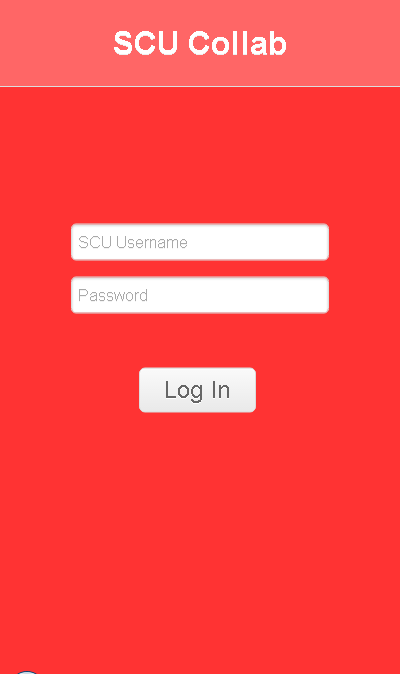
\includegraphics[scale=0.4]{images/login_screen.png}
	\caption{Login page}
	\label{fig:login screen}
\end{figure}

\begin{figure}[h]
	\centering
	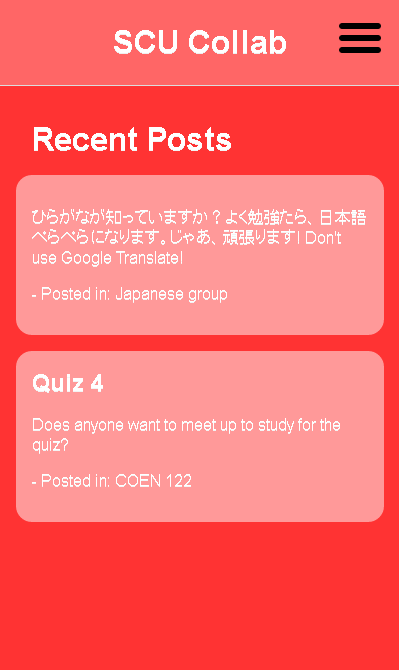
\includegraphics[scale=0.4]{images/home_screen.png}
	\caption{Home Screen}
	\label{fig:home screen}
\end{figure}

\begin{figure}[h]
	\centering
	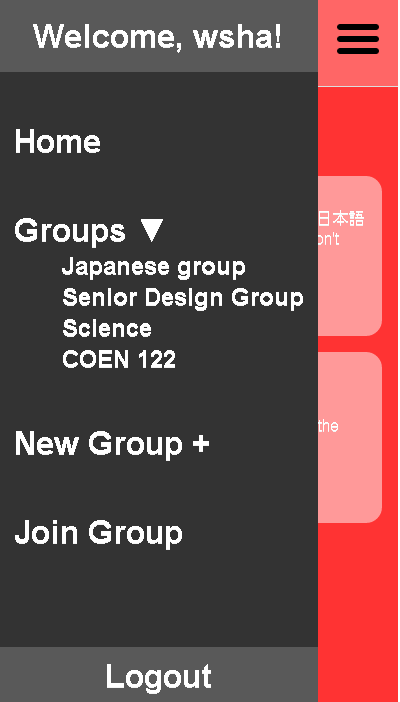
\includegraphics[scale=0.5]{images/sidebar.png}
	\caption{Sidebar}
	\label{fig:sidebar}
\end{figure}

\begin{figure}[h]
	\centering
	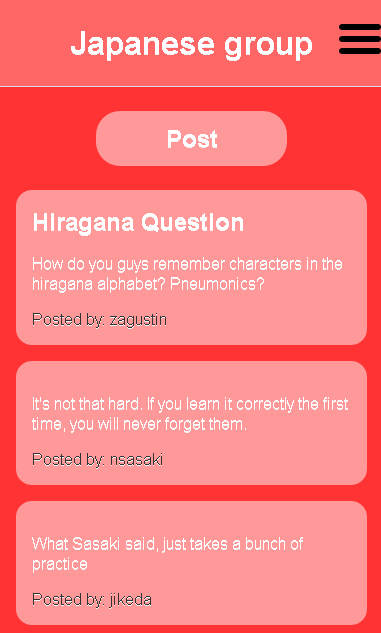
\includegraphics[scale=0.6]{images/group_pic.png}
	\caption{Group Page}
	\label{fig:group page}
\end{figure}
\chapter{Technologies Used}
As both a Web application and a hybrid mobile application, this application will be created using several such popular Web technologies. Several tools will be used to make this a reality.

\begin{itemize}
	\item HTML (Hyper Text Markup Language): HTML provides the main framework of the application. The functionality and styling of the application is built on top of the HTML file.
	\item CSS (Cascading Style Sheets): CSS is used to style HTML elements shown within the application.
	\item Javascript: JavaScript is used to provide interactive functionality for the sidebar in the application.
	\item PHP: PHP is a scripting language that provides functionality for the back end of the application.
	\item MySQL: MySQL is a relational database that stores information within data tables. This is hosted within the SCU web servers.
	\item JQuery Mobile: JQuery Mobile is a framework to streamline interface across various devices.
	\item Phonegap: Phonegap is a framework that allows for multi-platform hybrid applications.
\end{itemize}
\chapter{Architectural Design}
Figure 7.1 below shows how the technologies work with one another. On the client side, HTML and CSS provide the basic structure and styling. Javascript provides interactivity to the front end. JQuery Mobile also does some styling, but also provides an Ajax function. Ajax allows the application to make requests to the server side PHP files. PHP can then make requests to the database to send and retrieve information. The architectural design is shown in Figure 7.1 below.

\begin{figure}[h]
	\centering
	\includegraphics[width=\linewidth]{images/architectural_design.png}
	\caption{Architectural Design}
	\label{fig:architectural design}
\end{figure}
\chapter{Design Rationale}
The reason we use technologies such as HTML, CSS and Javascript is because they are essential Web technologies that are well documented, and simple to use. JQuery Mobile, in addition to its interface across different devices, was also used in consideration of Phonegaps' nature. Phonegap does not allow for server side files, so we needed to use AJAX which allows for asynchronous requests from the client side to server side. AJAX sends request to server, providing access to the server side PHP files. Jquery mobile has an AJAX method  built in, which helped us retrieve requests from the server. We use the MySQL database management system, which allows us to relate entities to each other, such as users to groups. This is one of the main relationships on our application. PHP had a large role in our system, as it was used to create group pages as well as interact with the database.

Many design decisions are made in order to enhance the usability of the application. The authentication system is based off SCU’s authentication systems, so students do not have to create new accounts, and ensures that only students can use the application. It also allows students more freedom and activity. The layout is kept simple since we have mobile devices in mind, and to limit visual distraction while maintaining user interaction. The sidebar is used to hide what is not being used. The forum is organized in a tabular format to keep the discussions organized.
\chapter{Testing}
\section{Unit Testing}
We tested the application as it was being made to ensure that all sections were working as intended. The functions that we wanted to ensure were working include the login features, the ability to join groups and communicate with groups members, and to access a calendar of events. We set up a number of test accounts and went through the various features.

\section{Integration Testing}
Once we confirmed that all units of the application were working properly, we integrated them into one and tested the application as a whole. We went through a comprehensive test of every unique page within the application to make sure there were no errors.

\section{User Testing}
After the application’s functionality was complete, we had other SCU students test the application. This acted as a stress test for our application by creating many test accounts and groups to see how well they could be handled.

Although students will likely create only a handful of groups with the application, we still created many instances of users and groups to test it.
\chapter{Lessons Learned}
Over the course of creating this application, our team has learned many tools and skills that will help us in the future in an engineering career.

\section{Workload Balance}
Work was split between working on the front end and the back end of the application. Most of the more intensive work resided with working on the backend, yet we did not give it special attention until the later stages of development. This most likely increased the amount of time it took to implement certain features in the application such as creating groups.

\section{Proper Research of Technologies}
While we had some previous experience with the core web technologies used in this application, we should have properly researched the technologies that were unfamiliar to us so that we could plan our design better. Rather than diving straight into the code, we should have taken extra time to understand our options, specifically for using Phonegap. More research would likely have allowed us to be more efficient with our development.

\section{Communication}
Throughout development, it became clear that communication between each of us was important. It helped us know how much progress each person has made, or when one of us needed help on a specific module or task. This affected us in the early stages of development since we mostly worked individually on our on tasks.
\chapter{Societal Issues}

\section{Ethical Justification}
The basis for this project is that all students should be able to receive help from others. However it can be difficult for certain student groups to set up meetings with others. For example, it can be inconvenient for commuters to meet up without prior planning. The purpose of our project is to allow students to easily collaborate with one another. We hope that this application will allow students to help one another either by using it to communicate with one another or organize meetings.

Figure 11.1 includes principles from the Software Engineering Code of Ethics that apply to the justification of our project:

\begin{figure}[h]
	\centering
	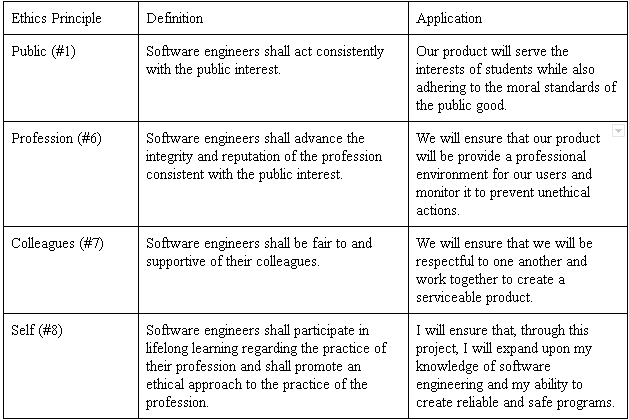
\includegraphics[scale=0.75]{images/ethics_table.png}
	\caption{Ethics Table}
	\label{fig:ethics table}
\end{figure}

\section{Organization}
Our project takes into consideration the availability of the web and how many devices are able to access it. We are aware that its availability will allow students to easily contact each other. Because of the availability of the internet, we want to encourage students to help each other succeed. We are also aware that this gives many different people access to our application and that it requires some sort of monitoring. 

In regards to our team, we realize that we need to work together in order to be more efficient. We are committed to having good communication so that we know that what we do is ethical and beneficial to our product.

\section{Effects on Society and Culture}
As with any platform that involves communication through the web, we need to be aware of the issue of cyberbullying. Because of application will provide a means for students to communicate with each other, it is also possible that users of malicious intent will harass others. Therefore, it is our duty to maintain a safe and friendly environment and ensure that our customers are free from any type of harassment.

Another ethical issue our product may come across is plagiarism or cheating. Because we want to create a platform where students can communicate with each other, this also allow them to share notes and other work. While we do believe this can be useful for student learning, it can also lead to cheating and/or plagiarism. I believe responsibility for this falls to both the product creators (my partner and me) and the user. The best my partner and I can do is limit the type of data that can be shared through our application. For example, we could restrict files or have a moderator (but that may prove to be difficult). However, it is also up to the users to avoid posting or copying the information that is shared.
\chapter{Conclusion}
Making SCU Collab a reality was a great undertaking that presented many challenges along the way. We learned a great deal about what working as a professional programmer would be like. From the satisfaction of creating our initial operating system, frustration at the accidental breaking of modules which took hours to fix, and our arrival at the final end product, we took away many valuable lessons from developing it. The greatest lesson we learned was by working as team on a simple concept, we could make systems that improve the lives of other people.

\section{Future Development}
While we completed the core functionalities of SCU Collab, there are some aspects that we would like to improve, specifically user management. As of now, there is no administrator or moderator role to oversee user activity. This lack of control may lead to unethical usage of the application as previously discussed in the ethical analysis. Other possible changes include improving overall usability based off user feedback.
\appendix

\chapter*{Appendix}

\section{Risk Analysis}
It is important to account for any risks that may happen during the development of this architecture. By establishing a contingency plan for common risks, hindrances within the development process will be minimized. The following risks can seen in Figure 12.1 below.

\begin{figure}[h]
	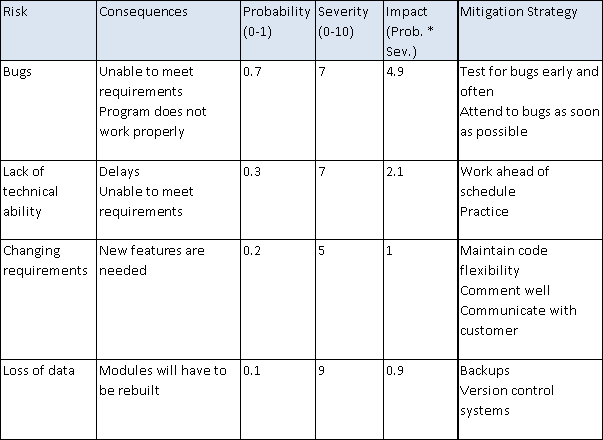
\includegraphics[width=\linewidth]{images/risk_analysis.png}
	\caption{Risk Table}
	\label{fig:risk table}
	\centering
\end{figure}

\clearpage
\newpage

\section{Development Timeline}
The development timeline shows a clear view of each team member’s responsibilities and roles in this project. Each team member’s progress can be traced across the time periods shown below in Figure 12.2.

\begin{figure}[h]
	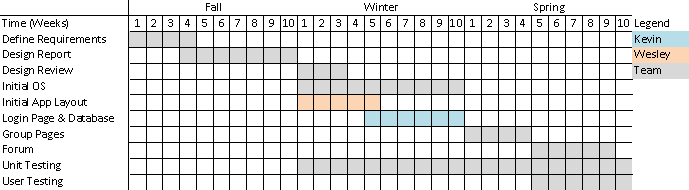
\includegraphics[width=\linewidth]{images/timeline.png}
	\caption{Development Timeline}
	\label{fig:timeline}
	\centering
\end{figure}

\backmatter
\end{document}
